\chapter{Evaluation\label{cha:evaluation}}

In this chapter the Orchestrator from chapter \ref{cha:orchestrator} is tested and evaluated. For this purpose an object detection application is used, which should be deployed to a given test infrastructure with several devices. In the first experiment the nodes join and leave the network one after the other. In the second experiment all nodes are online, but the network connection quality is manipulated. For both experiments it is examined which decisions the Orchestrator takes and what effect this decision has on the total latency of the application.

\section{Experimental setup}

\subsection*{Infrastructure}

\begin{figure}[htb]
    \centering
    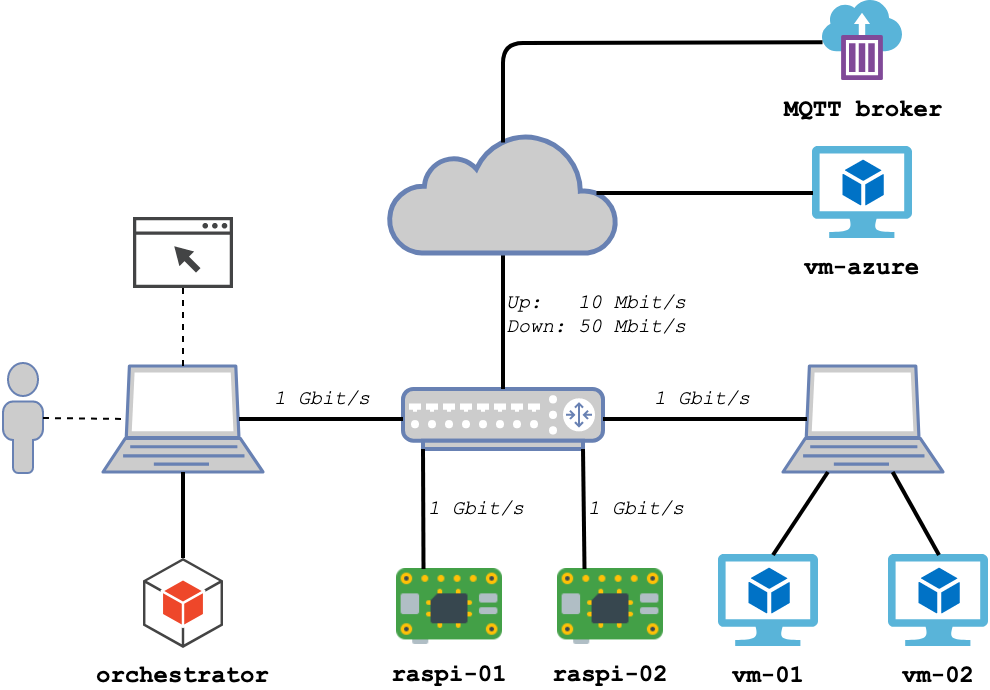
\includegraphics[width=0.85\textwidth]{evaluation-infrastructure}
    \caption{Test infrastructure for evaluation}
    \label{fig:evaluation-infrastructure}
\end{figure}

The test bed consists of the five nodes shown in figure \ref{fig:evaluation-infrastructure}. The hardware characteristics are shown in table \ref{tab:evaluation-devices}. The three virtual machines run Debian 10, the two Raspberry Pis run Raspbian 10. All nodes have \texttt{Docker} installed. Another device on the local network runs the Orchestrator and a web browser which can be used to access the \textit{Object Detection Web Application} and to evaluate the effect of the Orchestrators decisions. Communication between the nodes and the Orchestrator is done via an MQTT broker running in the Azure Cloud.

\begin{table}[htb]
    %\centering
    \begin{tabular}{|l|l|l|l|l|l|}
    \hline
        \textbf{Host} & \textbf{Device Type} & \textbf{CPU} & \textbf{RAM} \\
         \hline
         \texttt{raspi-01} & Raspberry Pi 3B+ & ARM Cortex-A53 1.4 GHz, 4 cores & 1 GB\\
         \hline
         \texttt{raspi-02} & Raspberry Pi 4B & ARM Cortex-A72 1.5 GHz, 4 cores & 4 GB\\
         \hline
         \texttt{vm-01} & Hyper-V VM & Intel i7-8550U 1.8 GHz, 2 vCPUs & 2 GB\\
         \hline
         \texttt{vm-02} & Hyper-V VM & Intel i7-8550U 1.8 GHz, 4 vCPUs & 4 GB\\
         \hline
         \texttt{vm-azure} & Azure VM \texttt{F4s\_v2} & Intel Xeon 2.7 GHz, 4 vCPUs & 8 GB\\
         \hline
    \end{tabular}
    \caption{Hardware characteristics of test devices used for evaluation}
    \label{tab:evaluation-devices}
\end{table}

\subsection*{Application}

\begin{figure}[htb]
    \centering
    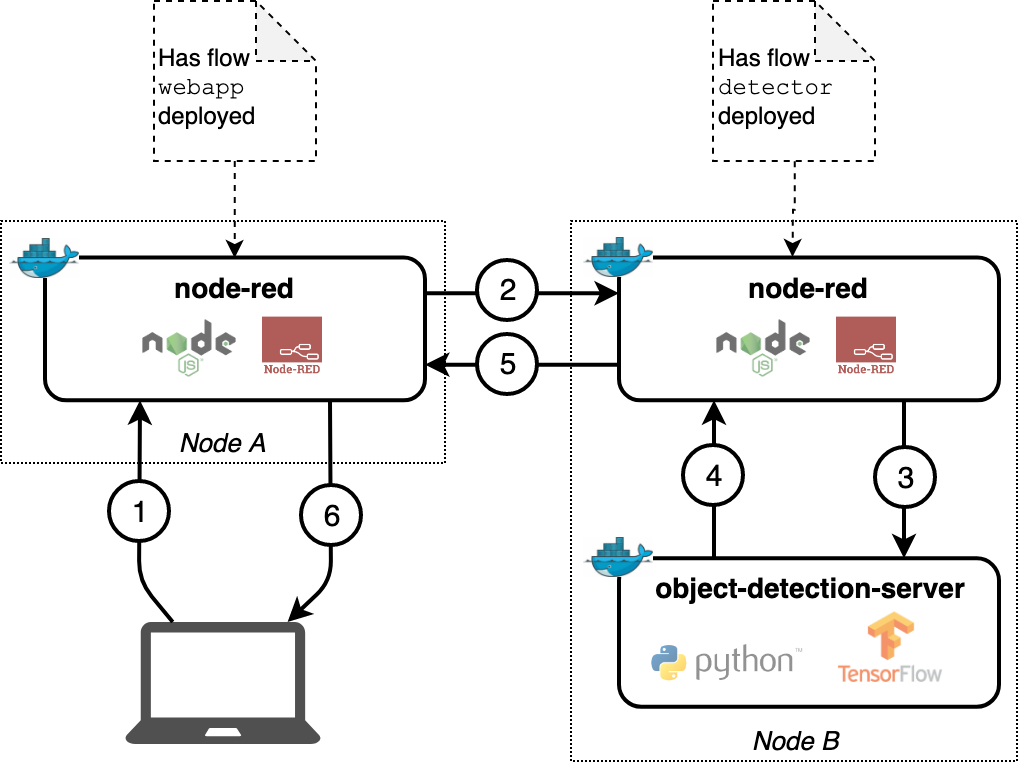
\includegraphics[width=0.85\textwidth]{evaluation-application}
    \caption{Object Detection Web Application} architecture
    \label{fig:evaluation-object-detection-application}
\end{figure}

The \textit{Object Detection Web Application} as shown in figure \ref{fig:evaluation-object-detection-application} consists of the two Node-RED flows \texttt{webapp} and \texttt{detector}. In the first step, a user sends an image for object detection to the \texttt{webapp} deployed on \texttt{raspi-01}. The user does not care on which node the object detection task is actually executed. The module \texttt{webapp} forwards the image for object detection to the module \texttt{detector} which is deployed on another node. This node can vary and is chosen by the Orchestrator. If a new node is selected by the Orchestrator, then the flow \texttt{webapp} will be updated so that the requests are forwarded to the new node.\\

The object detection engine can not be executed as a regular Node-RED flow, because Node-RED handles JavaScript functions only and the engine requires Python. Even if Node-RED could execute Python functions (there are extensions enabling this) the execution of the object detection engine in Node-RED would not be efficient because the engine would have to be initialized every time it is executed. However, the engine has a certain initialization time to load the detection graph. Therefore it is more efficient to initialize the engine only once at the beginning so that the following object detection tasks can be executed without additional initialization time. Because Node-RED can not initialize and hold Python objects, a separate docker container is used for this purpose. The flow \texttt{detector} sends an HTTP request containing the undetected image to the \texttt{object-detection-server} running on the same node. The server responds with the detected image which the \texttt{detector} then forwards back to the \texttt{webapp}.

There are three constraints:
\begin{enumerate}
    \item The flow \texttt{webapp} must be deployed on \texttt{raspi-01} because this is the only node known to the user
    \item The flow \texttt{detector} needs an \texttt{object-detection-server} container running on the same node
    \item The detected image must be available within 5 seconds
\end{enumerate}

\section{Orchestrator decisions and their impact on latency}

TODO

\section{Discussion}

TODO